\documentclass[conference]{IEEEtran}

\IEEEoverridecommandlockouts
\usepackage{cite}
\usepackage{amsmath,amssymb,amsfonts}
\usepackage{algorithmic}
\usepackage{graphicx}
\usepackage{textcomp}
\usepackage{xcolor}
\usepackage{fancyhdr}
\usepackage{lipsum}% generate text for the example

\def\BibTeX{{\rm B\kern-.05em{\sc i\kern-.025em b}\kern-.08em
    T\kern-.1667em\lower.7ex\hbox{E}\kern-.125emX}}
    
\fancypagestyle{firstpagefooter}{%
  \fancyhf{}
  \renewcommand\headrulewidth{0pt}
  \fancyfoot[R]{Forced-Directed List-Scheduling, Hamm-Lippstadt Hochschule}
}

\pagestyle{empty}

\begin{document}
\title{Forced-Directed List-Scheduling}

\author{\IEEEauthorblockN{Vytaras Juraska}
\IEEEauthorblockA{\textit{Electronics Engineering (6\textsuperscript{th} Semester)} \\
\textit{Hamm-Lippstadt Hochschule}\\
Lippstadt, Germany \\
vytaras.juraska@stud.hshl.de}
}

\maketitle

\begin{abstract}
an explanation and a deep dive on the theoretical concept of one of the heuristic scheduling algorithms called Force-Directed List-Scheduling, performance benchmarking and the toady's position of this unique scheduling solution. 
\end{abstract}


%\begin{IEEEkeywords}
%component, formatting, style, styling, insert
%\end{IEEEkeywords}

\thispagestyle{firstpagefooter}

\section{Introduction}

Design space exploration - the activity of exploring various design alternatives for the same physical amount of space, searching for the most optimal solution to a specific implementation. This problem has been the focus in numerous studies, and even though it is possible to formulate these problems using various methods (for instance Integral Linear Program), they quickly become unmanageable, unfit for the implementation, when the problem sizes get large. Much research has been done to address these problems have been with heuristic approaches, scheduling implementations, which do not focus on the most optimal solution, rather go for the prioritisation and lesser hardware resource usage, than maximum scheduling speed and full utilisation of hardware resources. 

A major motivation of the most popularly used Force-Directed Scheduling algorithm in the application of heuristic scheduling was to address the design space exploration task, that is, by performing Force-Directed Scheduling to solve a series of timing constrained scheduling problems. In a specific documentation\cite{b4}, the same authors, who invented Force-Directed Scheduling also proposed a method, called Force-Directed List Scheduling to address the resource constrained scheduling problem.

This specific scheduling algorithm is essentially an extension of an already mentioned Forced-Directed Scheduling algorithm. It adds an extension of List-Scheduling to the mentioned algorithm. Hence, in order to fully understand the Force-Directed List-Scheduling, both of its relevant parts have to be well defined.

\section{List-Scheduling Relevancy}

Relatively simple explanation of List-Scheduling (LS) (also refereed by Priority List Based Scheduling) is giving some sort of property to each of the component and defining a position of the component in a list corresponding to its properties unit. The conditions of the problem at hand are: having specified hardware constraints and trying to minimise the total time execution by using a local priority function to delay, or in other words - deffer, operations, which are at risk of creating recourse conflicts.

\subsection{Concept Definition}

Unlike ASAP (As Soon As Possible) and ALAP (As Late As Possible) scheduling algorithms, which processes each operation in a fixed order, LS processes each control step sequentially, choosing in before each step the best operation from all of the appropriate operations to place into the control step, while still depending on the resource constraints.

During the scheduling process, LS uses a ready list (hence the name) to keep track of data-ready operations. Data-ready operations are unscheduled operations the algorithm can schedule into the current control step while managing to upkeep the priority constraints (those operations whose immediate predecessors have been scheduled into earlier control steps). As long as the ready list contains data ready operations that meet the resource constraints, the algorithm chooses operations from that list and schedules them into the current control step. 

In choosing which ready-list operation to schedule, the algorithm sorts the ready list according to some priority function, always choosing the highest priority operation for scheduling into the current control step. One common priority function is based on mobility of operation - a variable, corresponding to the difference of the start times computed by the ALAP and ASAP algorithms, 
mathematical equation is as follows: 
\begin{equation*}
\displaystyle \mu_i = t_i^L - t_i^S; i = 0, 1, ..., n.
\end{equation*}
Zero mobility implies, that an operation can be started only at the given time step, hence operations with smaller mobility rate a higher priority, since there are fewer possible control steps into which those operations can be scheduled. Also, delaying them to a later control step would more likely increase the overall length of the schedule: this is especially true for those operations, which has the mobility of one.

The priority function selected clearly impacts the results of the list-scheduling algorithm - some systems give higher priority to operations with lower mobility, others give higher priority to operations with more immediate successors, stating that scheduling them in the current control step would make the largest number of operations data ready, thereby allowing the earliest possible consideration of each operation. Unfortunately, there is no agreement on which priority function is most optimal.

\subsection{Evaluation}

Overall, LS algorithm is so widely used, that majority of heuristic approaches were based from LS. Its low computational complexity makes it easily adaptable to bigger sized scheduling problems, where some more advanced heuristic scheduling approaches start gradually increasing their overall execution times, LS stays as a relatively quick algorithm. And in terms of smaller sized problems, other approaches have been shown not to differ much in latency. Hence, LS is a simple solution, which can be easily adapted to various situations.

\section{Force-Directed Relevancy}
Force-Directed Scheduling (FDS) was created in 1987 by Paulin and Knight, with an idea to find the most optimal and sufficient approach on how to minimise resource constrained scheduling problems (in real applications by reducing functional units, registers and buses), aiming for balanced overall concurrency of the operations, with having in mind of the design space exploration focus. To understand the working concept of the scheduling, its basic properties have to be defined.

\subsection{Basic Properties}

The time constrain has two variables, the earliest time variable and the latest time variable when the operation is expected to be executed, both of the variable form a, so called, time frame, which is defined as $\{[t_i^S, t_i^L]; i = 0, 1, ..., n\}$. This concept has been taken from and can be calculated with ASAP/ALAP algorithms, hence the corresponding naming of $t^S$ and $t^L$.

Probability of operations is defined as follows: outside the time frame it is zero, inside the time frame it is the reciprocal of the frame width. Hence the larger the width of the time frame, the lower the probability is for scheduled operation to be successfully executed in the corresponding time step. Mathematical representation of the probability of an operation at time $l$ is $\{p_i (l); i = 0, 1, ..., n\}$. So in this specific algorithm, it is required to not only have a limited time frame, but also the most optimal solution requires to keep the time frame as narrow as possible.

Lastly, a type distribution is the sum of probabilities of the operations, which are able to be implemented by a specific resource type at any time step. Mathematical definition of type distribution at time $l$ is $\{q_k (l); k = 1, 2, ..., n_{res}\}$. Using that we can create a distribution graph, which is a plot of an operation-type distribution over schedule steps. Distribution graph shows the probability of a specific resource being used in each scheduling step, while a so called uniform plot is a characteristic of a distribution graph, when operations are scattered evenly in the schedule, meaning that the utilisation of resource has been is done as efficiently as possible.

\subsection{General Representation of Force}

Having defined the basic properties of FDS, the main idea of the scheduling also has to be clarified - the idea of force. In FDS the selection of a candidate operation to be scheduled in a given time step is done using the concept of force. Forces attract and repel operations into and from specific schedule steps. For the sake of visualising the concept better, a force can be represented directly by the mechanical analogy - a force applied to an elastic spring is proportional to the displacement of both of its end points, hence the elastic constant is the proportionality factor. In FDS forces are related to how operations are grouped in certain control steps. Assigning an operation to a control step corresponds to changing its probability of execution, when the operation has been assigned to a certain step, at that step its probability is equals to 1, which means, that in any other step the probability of that operation is equals to 0. Hence coming back to the elastic spring analogy, the variation in probability is analogous to the displacement of a spring and the value of the type distribution given by the distribution graph at that step is analogous to the elastic constant.

Of course, the mechanical analogy is not a direct definition of this specific scheduling, FDS uses the forces and their probability to minimise the concurrency and still be able to fit in the fixed timing. The larger the force, the larger the concurrency. 

At every time step, each unscheduled operations probability is calculated, hence the operation with the smallest negative effect is selected. This probability is calculated as the force for an unscheduled operation at control step. There are two types of forces: self-force and predecessor-successor force and both of them are calculated differently.

\subsection{Mathematical Force Definition}
\subsubsection{Self-force}

Starting from the definition of self-force, let's consider operation $v_i$ of type $k = T(v_i)$ when scheduled in time step $l$. The force of an operation to a step $m \in [t_i^S, t_i^L]$ is equal to the distribution $q_k(m)$ times the variation in probability $1 - p_i(m)$. The self-force is the sum of forces relating the specified operation to all scheduled steps in its time frame, its mathematical definition is as follows:
\begin{equation*}
\displaystyle self-force(i, l) = \sum_{m=t_i^S}^{t_i^L} q_k(m) (\delta_{lm} - p_i(m))
\end{equation*}
where $\delta_{lm}$ represents Kronecker delta function, which states, that if the time step variable $l$ and operation force variable at that specific time step $m$ are equal, the $\delta_{lm}$ is equal to 1, if the mentioned two variables are not equal, the $\delta_{lm}$ is equal to 0.

Also, $p_i(m)$ may be defined as $\frac{1}{\mu_i + 1}$, when  $\forall m \in [t_i^S, t_i^L]$, where $\mu_i$ stands for mobility of the $i$ operation, hence the original expression can be represented as:
\begin{equation*}
\displaystyle self-force(i, l) = q_k(l) - \frac{1}{\mu_i + 1}\sum_{m=t_i^S}^{t_i^L} q_k(m)
\end{equation*}
\subsubsection{Predecessor-Successor Force}

Once an operation is set to a specific step, time frame of other operations may reduce, hence after setting the operation, predecessor-successor forces, which are forces on other operations linked by dependency relations, have to also be considered and if needed, recalculated.

Predecessor-successor forces are computed by evaluating the difference between predecessor-successor force and self-force, considering the restriction of their time frames. Mathematically defining the initial time frame to be $[t_i^S, t_i^L]$ and the reduced time as $[\tilde{t_i^S}, \tilde{t_i^L}]$ and using the previously defined formula of self-force, the predecessor-successor force expression is defined as follows:
\begin{equation*}
\displaystyle ps-force(i, l) = \frac{1}{\tilde{\mu_i }+ 1}\sum_{m=t_i^S}^{\tilde{t_i^L}} q_k(m) - \frac{1}{\mu_i + 1}\sum_{m=t_i^S}^{t_i^L} q_k(m) 
\end{equation*}
Hence, to calculate the total force of an operation related to the schedule step it is required to add the operations self-force with all of its predecessors and successors forces, of which their time frame is affected.

\subsection{Issues Introduced}

As good as FDS may seem, its methods introduce some issues, which might be problematic in certain applications. FDS is designed so that every decision is made with a greedy manner, so there is no guarantee, that the solution will be the most optimal. One of the biggest reasons, is that FDS considers the operations one at a time, instead of the strategy of considering each schedule step at a time (as done by LS). 

Continuing on, if FDS locates two potential assignments with the same cost, it will not be able to accurately estimate the best choice. And lastly, the computational complexity drastically increases with having more operations to manage, since there are various of iterations as operations and each of them requires separate calculations of forces. Even though FDS truly works well on smaller sized problems, it really struggles on bigger ones, so much so, that this scheduling approach is considered inferior, with regards to bigger sized problems.

\section{Force-Directed List-Scheduling}

As mentioned in the introduction, Force-Directed List-Scheduling (FDLS) is an addition of LS to FDS, which both of them were already defined in previous sections. The conditions of the problem, which the FDLS is solving, are similar to FDS, but where as FDS, as described by the authors, is more focused on fixed latency constraints, FDLS is meant to be focused on fixed resource constraints, while also having limited time frame of the operation and going for the near-minimum value of total execution time, considering that the scheduling is still a heuristic approach. It was also created by Paulin and Knight, and where as FDS aims for the similar problem, FDLS generally was the more optimal solution, since FDS has some flaws in areas, where FDLS goes through some of them without issues.

\subsection{Concept Definition}

Generally, the main concept is to adapt the idea of global measure of concurrency from FDS throughout the scheduling process and adapt it to the process of deferring operations from LS, if they are about to cause recourse conflicts. 

In previously described LS, the selection of the deferred operations is determined by a local priority function such as urgency or mobility. In FDLS, the approach is similar, except that force is used as the priority function, which means, that whenever a hardware constraint is exceeded when the scheduling of LS is taking place, force calculations are used to select the most suitable operations which have to be deferred. Here, a deferral does not necessarily mean that the operation will be scheduled in the next control step, only that its time frame has been reduced since the FDLS already knows, that the specific operation is not suitable for that control step. The deferrable operation that produces the lowest force, which means the lowest global measure of concurrency increase, is chosen. This is repeated until the hardware constraint is met.

In terms of the force calculation, the same methods are applied, which are already described in FDS. Although the only difference is the global time constraint, which in the case of FDLS, is set to be the current critical path - the longest scheduling path, which is still in the limited time frame. The length may be increased when the only way of solving an operation which is raising a recourse conflict, is to defer a critical operation.

\section{Benchmarking and Appliance}

\subsection{Benchmarking Results}

\begin{figure}[htbp]
\centerline{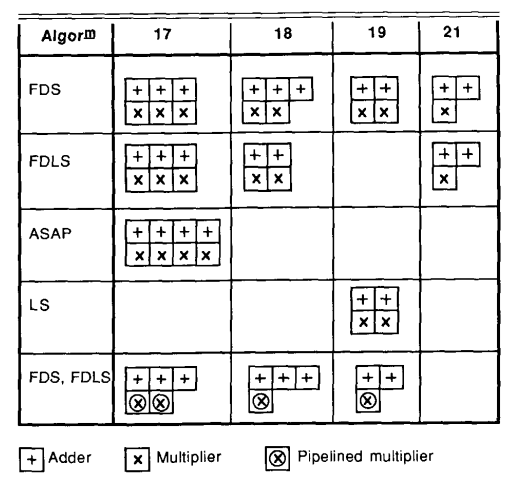
\includegraphics[scale=.5]{Result_Applience.png}}
\caption{Fifth-Order Wave Digital Elliptic Filter Results}
\label{wavefilter}
\end{figure}

Originally, in a specific documentation \cite{b2}, Paulin and Knight used an already existent method of benchmarking, with which they tested the performance of various scheduling algorithms, with a so called implementation of a fifth-order wave digital elliptic filter. This is a computationally lengthy task, which requires 43 operations (additions and multiplications), hence it is a great tool to, in a sense, stress test the algorithms efficiency and since this method has been already used in other studies, it creates an opportunity of comparison with other studies.

Since the topic at hand is FDLS, the only relevant algorithms are FDLS and FDS, unfortunately LS benchmarking was not as significantly different and well defined in the original documentation, hence LS results will also be ignored.

Paulin and Knight acknowledges, that multiplications require two times more time, than additions, hence multiplication operation took two control steps, while addition took only one. The calculated overall critical path is 17 control steps. The first row from the top of the Figure \ref{wavefilter} represents the different timing constraints, while the first column from the left side are the names of algorithms, to which this benchmark was applied. In the rest of the fields, we can see the direct amounts and types of operations, which each of the algorithm produced, at  specific times constraint, to solve the scheduling problem of executing fifth-order wave digital elliptic filter efficiently.

\subsubsection{Force-Directed Scheduling}

Taking a look at the results of FDS, we can see the specific solutions found by the FDS on time constraints being: 17, 18, 19, 21. According to Paulin and Knight, during this benchmark the CPU run times varied between two and six minutes.

\subsubsection{Force-Directed List-Scheduling}

This specific benchmark was obtained by taking the FDS results with the time constraints of 17, 19 and 21, setting the maximum limit of required functional units and running the FDLS algorithm. Surprisingly, for the time constraints 17 and 21, the results were already optimal enough, so the time was not reduced. However, at the time constraint of 19 control steps the FDLS algorithm produced a solution, which had one control step less, than FDS algorithms initial result, hence this solution is also considered to be the optimal solution and it can not be further improved. 

Even if the results were not very different, the CPU run times were significantly faster, than FDS. On this benchmark it varied between one and two minutes.

According to Paulin and Knight, the improved time over constraint of 19 control steps is mostly due to the fact, that they have described the constraint of functional units and dedicated the time constraint, where as on FDS benchmark, only the time constraint was given. Also, FDLS has significantly less force calculations, rather than FDS, hence the CPU run times were much lower this time.

\subsection{Force-Directed List-Scheduling applied in a Digital Microfluidic Biochip}

Digital Microfluidic Biochip (DMFB) is an emerging technology, that aims to miniaturize and integrate droplet-based functions into a chip by manipulating droplets with various sized volume. Droplets are small sized liquid bubbles, which, in terms of DMFB, can be used to apply them to digital applications. DMFB provides higher sensitivity and less human error compared to other benchtop chemistry implementations.

A small group of people: Kenneth O'Neal, Daniel Grissom, Philip Brisk - wrote an interesting documentation \cite{b5}, where they considered applying FDLS algorithm to DMFB. Once applied, they noticed, that this implementation is the most efficient way to schedule droplet-based scheduling. But since the implementation of FDLS is already quite outdated, since there are already modified versions of this specific scheduling algorithm, which perform, depending on the implementation, better.

Never the less, since FDLS is more focused on scheduling problems based on resource constraints, and in DMFB there is definitely a significant lack of resources, compared to standard quantity of electronic based computational resources, purely caused by the size of droplets and the maximum possible speed of each droplet, the computational resource constraint is the biggest focus, when considering scheduling in DMFB. And the ability of FDLS to still maintain fairly short execution times, definitely adds to the title of the most efficient scheduling approach in the field of DMFBs.



\section{Advantages}
When using the correct approach successfully, the advantages of combining both of the mentioned scheduling algorithms, their individual advantages are kept:

\begin{itemize}
\item High utilisation of functional units, this originally comes from the LS;
\item Low computational power complexity;
\item Operations are evaluated globally before their assignment to the control step.
\end{itemize}

\section{Disadvantages}
Since FDLS is still a heuristic scheduling algorithm, it is definitely not a one solution for all of the scheduling problems. The reality is, that each problem is solved the best by the most specific implementation. Hence in terms of execution times, FDLS is definitely not the most optimal solution.

Even if the computational power complexity is low, force calculations is an extra step added to the LS, where this algorithm is already performing quite well on its own, being capable of even quicker execution times. So the bigger the scheduling problems - the more computational power FDLS required, compared to LS.

Paulins and Knights implementation of FDLS already has slight improvements done by other people, it is still a widely used algorithm, but there are definitely better options out there.

\section{Conclusion}
This unique scheduling approach, combining different concepts from two different algorithms, definitely shows, that in terms of heuristic scheduling solutions, there can be always room for improvement. Even if FDLS is a relatively outdated solution by today's standards, there are many interesting technological enhancements which can still easily use the concept of FDLS and receive quick and computationally light results, with the ability of adapting the concept to a specific problem.

\begin{thebibliography}{00}
\bibitem{b1} 
Micheli, G. De (1994). Synthesis and Optimization of Digital Circuits. McGraw-Hill, New York.
\bibitem{b2} 
Paulin, P. G. and Knight, J. P. (1989). Force-directed scheduling for the behavioral synthesis of asic’s. IEEE Transactions on Computer-Aided Design, 8:661–679.
\bibitem{b3}
R. A. Walker and S. Chaudhuri, "Introduction to the scheduling problem," in IEEE Design & Test of Computers, vol. 12, no. 2, pp. 60-69, Summer 1995, doi: 10.1109/54.386007.
\bibitem{b4}
Paulin, P. G. and Knight, J. P. (1987). Force-directed scheduling in automatic data path synthesis. In 24th ACM/IEEE conference Proceedings on Design Automation Conference.
\bibitem{b5}
K. O'Neal, D. Grissom and P. Brisk, "Force-Directed List Scheduling for Digital Microfluidic Biochips," 2012 IEEE/IFIP 20th International Conference on VLSI and System-on-Chip (VLSI-SoC), 2012, pp. 7-11, doi: 10.1109/VLSI-SoC.2012.7332068.
\end{thebibliography}

\end{document}
